%------------------------------------------------------------------------------------------------------------------------------------------
% Navrhy
%------------------------------------------------------------------------------------------------------------------------------------------
\chapter{VLASTNÍ NÁVRHY}
\par Nástroj, který je součástí této práce se zaměří z velké části na uživatelské rozhraní a do jisté části využije technologie a nástroje, které jsou dostupné a usnadní takto vývoj a nasazení tohoto nástroje. Dále se zaměříme na životaschopnost tohoto nástroje a způsobu jakým bude takto vytvořený nástroj nabízen veřejnosti. Rozsah firem, pro které bude tato aplikace doporučována je malé, až střední podniky, které pracují s větším množstvím dat a potřebují nějakým způsobem najít skryté informace.

\section{Návrh aplikace}
\par Aplikace je postavena na základě aplikačního serveru WildFly, který pracuje s moduly napsanými v jazyce Java. Základní rozdělení aplikace je tedy \textbf{Engine} a \textbf{UI}, engine je připojen na databázi MongoDb, což je NoSql databáze. Výhodou tohoto nastavení je vysoká pružnost v rámci zapsaných dat a není tedy nutné přesně definovat závislosti v rámci databáze (každý zákazník si může definovat jiné důležité atributy pro každý projekt).
\par Další výhodou oddělení uživatelského rozhraní a samostatného enginu je možnost lépe řídit vývojářský tým, lépe rozdělit práci a v neposlední řadě, také možnost později vytvořit klienta nezávislého na dosavadním uživatelském rozhraní -- například vytvoření mobilní aplikace, která se bude specializovat na určitou část systému. Celý systém spolu komunikuje tedy pomocí REST rozhraní a o zabezpečení se stará vrstva Keycloak, ve kterém jsou oba moduly registrovány a slouží jako takový středobod celého systému. Jak jsou jednotlivé části propojeny můžete vidět na obrázku \ref{schema}, kde hrany znamenají komunikační zprávy a uzly logické bloky.

\begin{figure}[!htp]
\centering
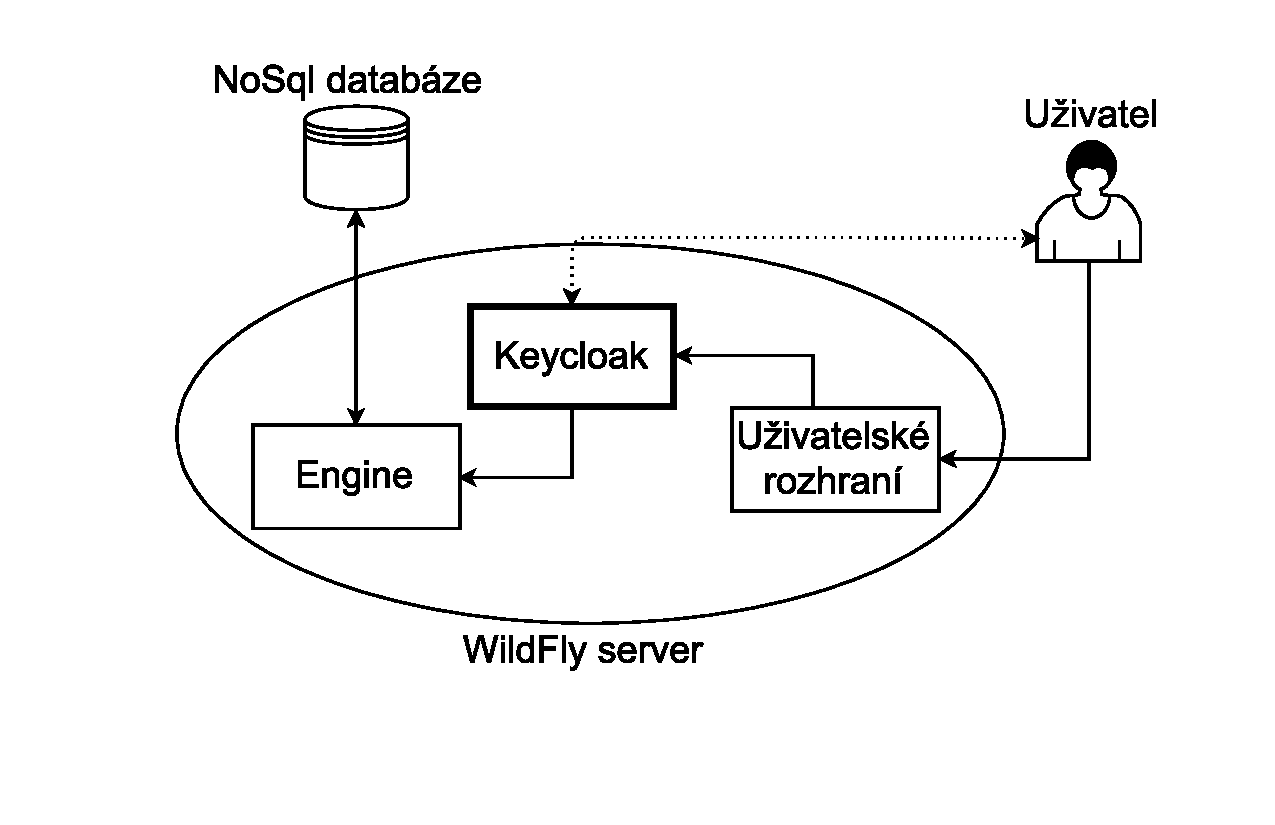
\includegraphics[max size={\textwidth}]{navrh.pdf}
\caption{Diagram znázorňující schéma nástroje.}
\label{schema}
\end{figure}

\par Pro znázornění jak dochází k získání dat se můžeme podívat na diagram \ref{komunikace}. Kde uživatel vyvolá jakoukoliv akci, která vyžaduje získání dat ze serveru, uživatelské rozhraní se nejdříve zeptá Keycloak serveru, zda má aktivní token stále aktivní a pokud ne, autentizační server mu vytvoří nový. Poté uživatelské rozhraní pošle dotaz na samotný engine (v tomto dotazu se nachází autentizační token), kde se zkontroluje opět životnost tokenu a zda má uživatel práva pro daná data. Pokud je vše v pořádku server vrátí data, pokud ne odpoví chybovou hláškou. Výhodou takovéto komunikace je, že nezáleží na implementaci uživatelského rozhraní, to může být napsáno jak pomocí webových technologií (Javascript), tak jako mobilní aplikace.

\begin{figure}[htp]
\centering
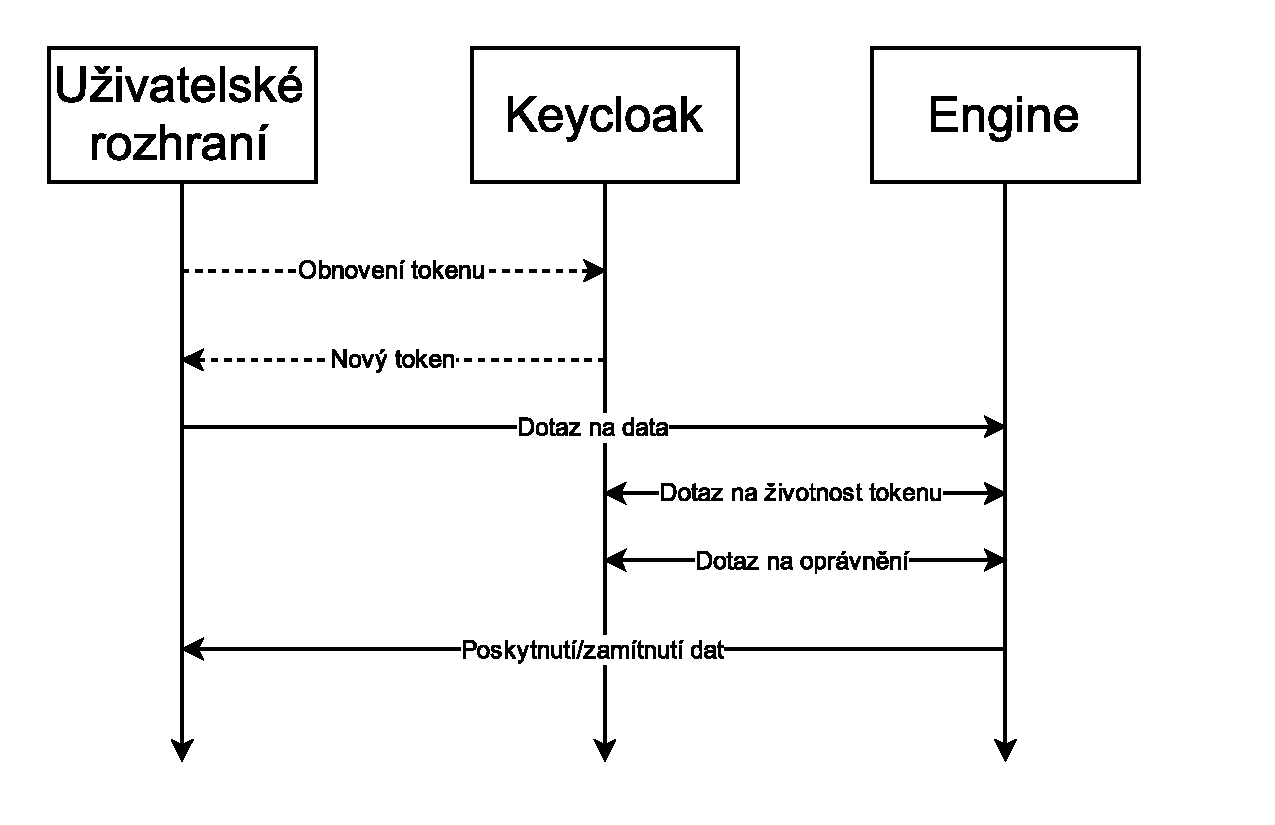
\includegraphics[max size={\textwidth}]{komunikace.pdf}
\caption{Diagram znázorňující schéma nástroje.}
\label{komunikace}
\end{figure}

\par Pokud uživatel již disponuje velkým datovým uložištěm je ho možné připojit do systému jednoduchou konfigurací v rámci UI, systém prozkoumá tyto data, některá si nakopíruje a začne je uživateli nabízet podobně, jako kdyby je uživatel měl již dříve v systému. Podobně je tomu s dolováním dat -- modul, který je zodpovědný za samostatné dolování je možné připojit do systému, odkázat jej na datové uložiště a spustit samostatné dolování dat. Vše je nastavitelné jak z uživatelského prostředí, tak pomocí volání na předem definované RESTové služby.

\subsection{Vedení vývojového týmu}
\par Pro snadný a rychlý vývoj bylo nutné zvolit vhodné vedení vývojového týmu, který se podílel na vývoji celé aplikace. Ze zkušeností bylo určeno že rychlého vývoje se dosáhne použitím agilní metody vedení týmu, inspirováno scrumem. Nicméně, protože jednotliví členové týmu se nenacházeli v dostatečné vzdálenosti a nebyl tento projekt veden jako hlavní úkol jednotlivých členů, některé setkání, která jsou definována ve scrumu byla vyškrtnuta. Nejenom proto nelze vedení týmu, které bylo zvoleno označit jako čistokrevný scrum, ale pouze že jsme se při vedení inspirovali touto metodikou.

\par Nastavili jsme si třítýdenní zveřejnění jednotlivých částí a každý týden jsme se scházeli abychom si ujasnili na čem jaký člen týmu dělá a zda nemá nějaký problém. Použili jsme také nástroje určené ke snadnějšímu rozdělování práce, kdy jsme začali s používáním nástroje \textbf{Trello}\footnote{Jednoduchý nástroj, který vizualizuje aktuální práci za použití jednoduchých tabulí \url{https://trello.com/}.}, který nám postupně přestal stačit a tak jsme využili opensource licence \textbf{Youtrack}\footnote{Tento nástroj je podobný Trellu, nicméně dovoluje snadnější a pro tým důležitou vizualizaci práce \url{https://www.jetbrains.com/youtrack/}.}

\subsection{Popis aplikační funkčnosti}
\par Před samotným popisem co a jak je propojeno si musíme určit co vlastně bude tato aplikace dělat a důvod jejího vzniku. Hlavním důvodem vzniku této aplikace je usnadnění editace často složitých záznamů (souborů) pomocí moderních technologií, záznamy můžeme rozumět například tabulky, grafy, kontingenční tabulky, atd. Mezi jednotlivými záznamy mohou vznikat a zanikat propojení, které umožní snadné napovídání datových záznamů a popisu dat (v případě tabulky si toto lze představit že nám aplikace bude napovídat možné záhlaví tabulky a data v tabulce). Editace a nahlédnutí do záznamů bude povolena pouze určitému uživateli. Dále jednotlivé soubory bude uživatel moci seskupovat do takzvaných kolekcí, tímto dosáhneme jisté abstrakce nad soubory, tak aby uživatel přibližně tušil již při prvním pohledu na záznam jaká data v něm mohou být. Vzhledem k tomu, že aplikace bude cílena na větší množství uživatelů aplikaci je možné přepínat mezi různými projekty a organizacemi, takže uživatel může mít několik záznamů se stejným jménem ve stejné kolekci pod různými projekty a organizacemi.

\section{Použité technologie}
\par Může se zdát že pro vytvoření tohoto nástroje bylo použito velké množství technologií, proto se následující kapitola bude věnovat jednotlivým částem aplikace. Jaké technologie přesně používá, jak jsou tyto technologie propojeny a k čemu je to dobré.

\subsection{Engine}
\par Základní část celé aplikace a její středobod se skládá ze tří pomyslných částí \textbf{Databáze}, \textbf{REST rozhraní} a \textbf{hlavní logika}. Díky tomuto rozdělení je možné snadně a hlavně rychle přidat novou funkcionalitu, dále je také možné rozdělit jednotlivé části vývojářům, kteří se mohou zaměřit na menší úkoly a pracovat tak efektivněji.

\par Hlavní logika byla naprogramována v jazyce Java a jako aplikační server poté Wildfly, díky jeho snadnému propojení do Keycloaku a převážně díky jeho robustnosti -- největší předností je jednoduché napojení na velké množství různých databází. K načtení závislostí, sestavení a nasazení tohoto modulu byl použit nástroj Maven. V podstatě pro jednoduchost si můžeme představit jako vstup databázi a jako výstup RESTové rozhraní.

\begin{itemize}
\item \textbf{Databáze} postavena nad technologií NoSql, MongoDb. V pozdějším použití budeme pravděpodobně muset sáhnout po nějakém indexovacím nástroji, jako je například Elasticsearch, nebo Solr, který nám umožní snadnější hledání napříč složitější databázovou strukturou.
\item \textbf{REST rozhraní} nástroji slouží pro snadnější přístup k jednotlivým datům a definuje snadno dostupné koncové uzly. Pokud bude potřeba nástroj rozšířit a hlavně zmapovat jednotlivé koncové uzly budeme moci použít například technologii Swagger\footnote{Slouží pro vizualizaci a zobrazení jaké data jednotlivý uzel očekává a jaké produkuje \url{http://swagger.io/}.}
\end{itemize}

\subsection{Uživatelské rozhraní}
\par Vzhledem k tomu, že hlavní část aplikace je nasazována na aplikační server Wildfly, také uživatelské rozhraní je sestaveno a možno nasadit jako samostatný modul. Samotný proces sestavení používá nástroj \textbf{Webpack}, který celý zdrojový kód rozdělí do dvou Javascriptových souborů. Jeden obsahuje závislosti nutné pro chod aplikace a druhý obsahuje samostatný kód aplikace. V rámci usnadnění a jednoduššího přístupu k aplikaci jsme se rozhodli velkou část Javascriptových souborů umístit na veřejné CDN\footnote{CDN je v podstatě systém serverů, které nabízejí JS a CSS soubory uživatelům s ohledem na jejich geografickou lokaci, tak aby měli tyto soubory co nejdříve.}.

\par Vzhledem k rozsáhlosti a složitosti uživatelského rozhraní bylo rozhodnuto, že se použije aplikační framework s podporou jednostránkové aplikace, po prozkoumání alternativ byl následně vybrán rámec \textbf{Angular 2}. S výběrem tohoto aplikačního rámce jde ruku v ruce také výběr jazyku ve kterém je uživatelské rozhraní napsáno, což je silně typovaný jazyk \textbf{Typescript}.

\par Uživatelské rozhraní se postupně upravovalo a byla snaha o co možná nejjednodušší používání této aplikace, proto byla první verze rozhraní představena několika méně zkušeným uživatelům počítače, kterým se dali jednoduché úkoly a byl sledován jejich postup a následně jim byla položena otázka zda byl úkol snadný. Systém jim byl pouze zevrubně vysvětlen slovy, že se jedná o aplikaci, která obsahuje kolekce souborů, které jsou mezi sebou propojeny. Jak vypadalo uživatelské rozhraní před těmito úkoly se můžete podívat na obrázku \ref{old-ui}.

\begin{figure}[!h]
\centering
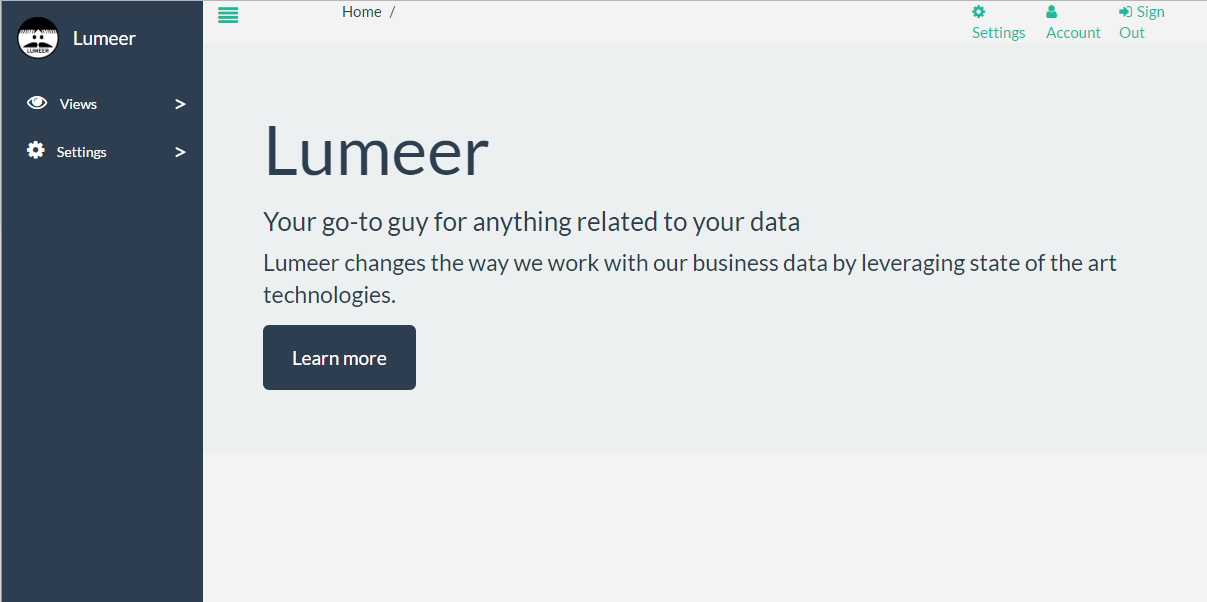
\includegraphics[max size={\textwidth}]{old-design}
\caption{Design aplikace před představením uživatelům.}
\label{old-ui}
\end{figure}

\subsubsection{Úkol číslo 1} Výběr kolekce a následně zjištění informací o této kolekci. Úrověň náročnosti \textbf{lehká}, na výsledky hodnocení se můžete podívat v tabulce \ref{ukol-1}.
\begin{table}[htp]
\begin{center}
\begin{tabular}{ || c || c | c | m{5cm} || }
\hline
Číslo uživatele & Rychlost vykonání & Ohodnocení & Slovní popis \\ [0.5ex]
\hline
\hline
1 & 25s & Snadný & Úkol se mi zdál ze začátku těžký, ale postupně jsem přišel na to kam kliknout. \\
\hline
2 & 38s & Středně těžký & Úkol se mi zádl celkem těžký a byl jsem docela zmatený s aplikací. \\
\hline
3 & 43s & Těžký & Vlbec jsem nechápal kam kliknout a potřeboval jsem pomoc. \\
\hline
\end{tabular}
\end{center}
\caption{Vyhodnocení úkolu číslo 1.}
\label{ukol-1}
\end{table}
\subsubsection{Úkol číslo 2} Výběr kolekce a dokumentu v kolekci pro který budou upraveny propojení. \textbf{středně těžká}, na výsledky hodnocení se můžete podívat v tabulce \ref{ukol-2}.
\begin{table}[htp]
\begin{center}
\begin{tabular}{ || c || c | c | m{5cm} || }
\hline
Číslo uživatele & Rychlost vykonání & Ohodnocení & Slovní popis \\ [0.5ex]
\hline
\hline
1 & 40s & Středně těžký & I po předhozím pochopení aplikace jsem měl s aplikací celkem problém.\\
\hline
2 & 48s & Těžký & Vůbec jsem něvěděl kam kliknout a co dělat. \\
\hline
3 & 1m 15s & Těžký & Potřeboval jsem hned od začátku pomoci a potřeboval jsem úkol několikrát vysvětlit a pomoci co dělat. \\
\hline
\end{tabular}
\end{center}
\caption{Vyhodnocení úkolu číslo 2.}
\label{ukol-2}
\end{table}
\subsubsection{Úkol číslo 3} Výběr kolekce a dokumentu v kolekci pro který se zobrazí práva. Úroveň náročnosti \textbf{těžká}, na výsledky hodnocení se můžete podívat v tabulce \ref{ukol-3}.
\begin{table}[htp]
\begin{center}
\begin{tabular}{ || c || c | c | m{5cm} || }
\hline
Číslo uživatele & Rychlost vykonání & Ohodnocení & Slovní popis \\ [0.5ex]
\hline
\hline
1 & 30s & Středně těžký & Vzhledem k tomu že tento úkol navazoval na předešlý, hned jsem věděl kde přibližně hledat. \\
\hline
2 & 52s & Těžký & Úkol navazoval na druhý a proto jsem přibližně věděl co a kam kliknout. \\
\hline
3 & 1m 10s & Těžký & Úkol byl podobný jako druhý úkol a proto jsem nepotřeboval takovou pomoc. \\
\hline
\end{tabular}
\end{center}
\caption{Vyhodnocení úkolu číslo 3.}
\label{ukol-3}
\end{table}

\par Vzhledem na výsledky hodnocení a uživatelské podněty se tým rozhodl přepracovat UI do více uživatelsky přívětivého způsobu. Hlavní výtka všech uživatelů bylo příliš mnoho navigačních prvků na stránce, což vede k nepřehlednosti a uživatelé tak nevědí na co kliknout a co použít. Na druhou stranu většina uživatelů, kterým byla aplikace představena zdůraznili výhodu vyhledávání a filtrování v rámci kolekcí, dokumentů a propojení. Z těchto poznatků bylo tedy určeno, že nejlepší bude zvýraznit vyhledávací formulář, který bude na všech stránkách aplikace. Dále také nějakým způsobem sjednotit všechny prvky aplikace do jednoho vyhledávání, tak aby uživatelé měli přehledně a snadno dostupné například dokumenty a hned vedle nich propojení. Z těchto požadavků bylo tedy navrhnuto nové uživatelské rozhraní, které lze vidět na \ref{new-ui}.

\begin{figure}[htp]
\centering
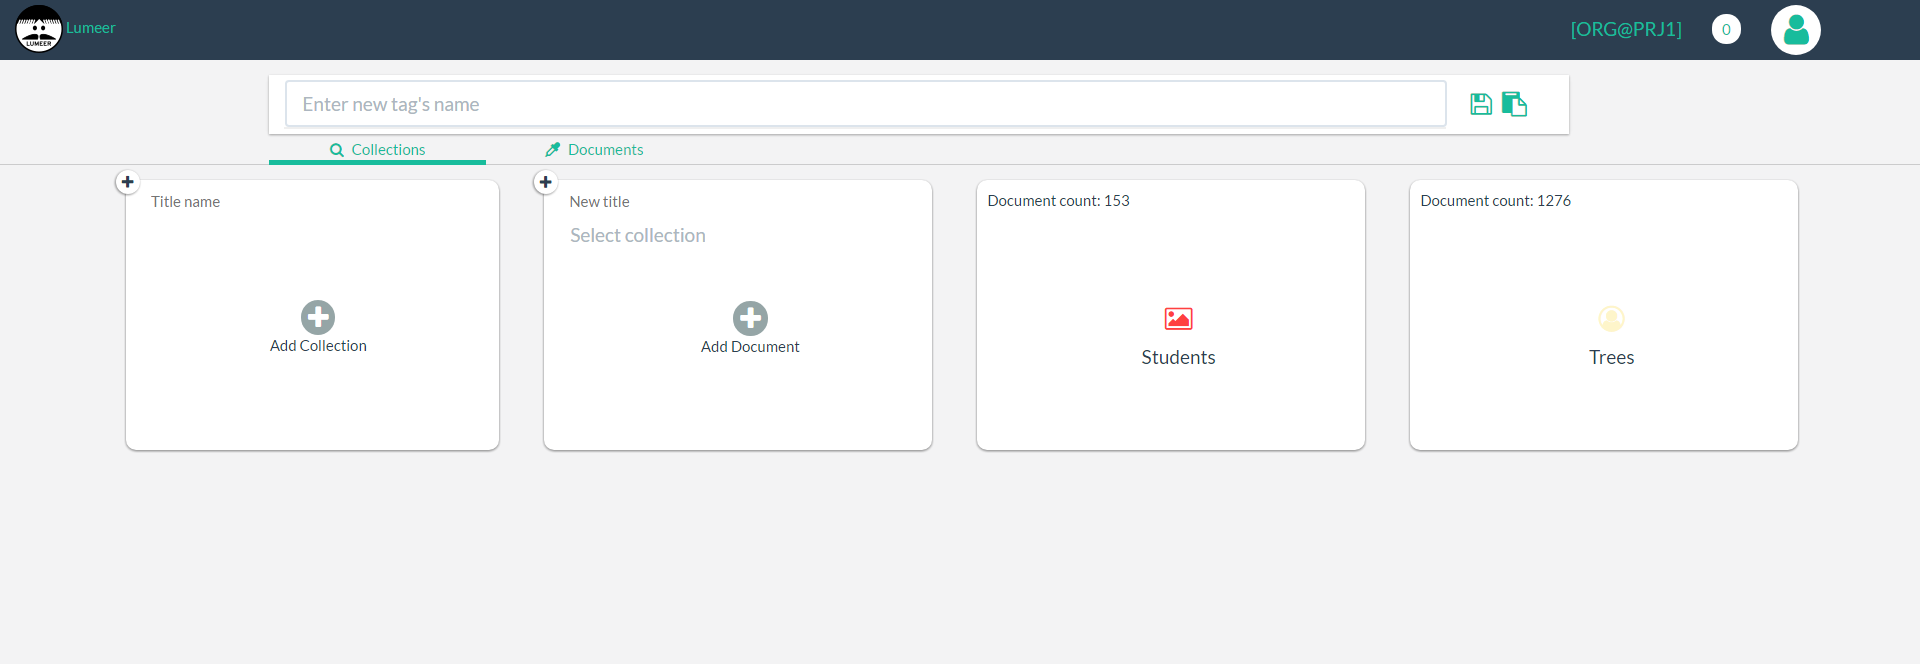
\includegraphics[max size={\textwidth}]{new-design}
\caption{Návrh nového uživatelského rozhraní.}
\label{new-ui}
\end{figure}

\subsection{Práce s grafy}
\par Díky tomu, že využíváme webové technologie můžeme jednoduše vytvořit grafy, pro znázornění některých datových sad. Aplikace využívá více knihoven pro práci s daty, aby umožnila uživateli jednoduchou práci a možnost měnit typ grafů, upravovat datovou sadu atd.

\subsubsection{Jednoduché grafy}
\par Pro znázornění a práci s jednoduchými grafy jsme využili knihovny \textbf{chart.js}, tato knihovna se snadno ovládá a je jednoduchá pro nastavení, nicméně složitější grafické útvary nejsou jednoduché na vytvoření. Základní uživatel disponuje několika druhy grafů z této knihovny. Pokud chce používat složitější grafické znázornění musí si více připlatit a v aplikaci se zpřístupní možnost používat složitější grafy, které jsou vytvořeny v knihovně \textbf{D3}. V základních operacích s grafy nabízí aplikace jednoduché sloupcové, spojnicové, koláčové a radarové grafy. Uživatel si může zvolit z jakých datových sad bude čerpat data, jak je namapuje na grafy a případně možnost exportu grafu do pdf a obrázku.
\begin{figure}[!htb]
\centering
\subfloat[Sloupcový]{{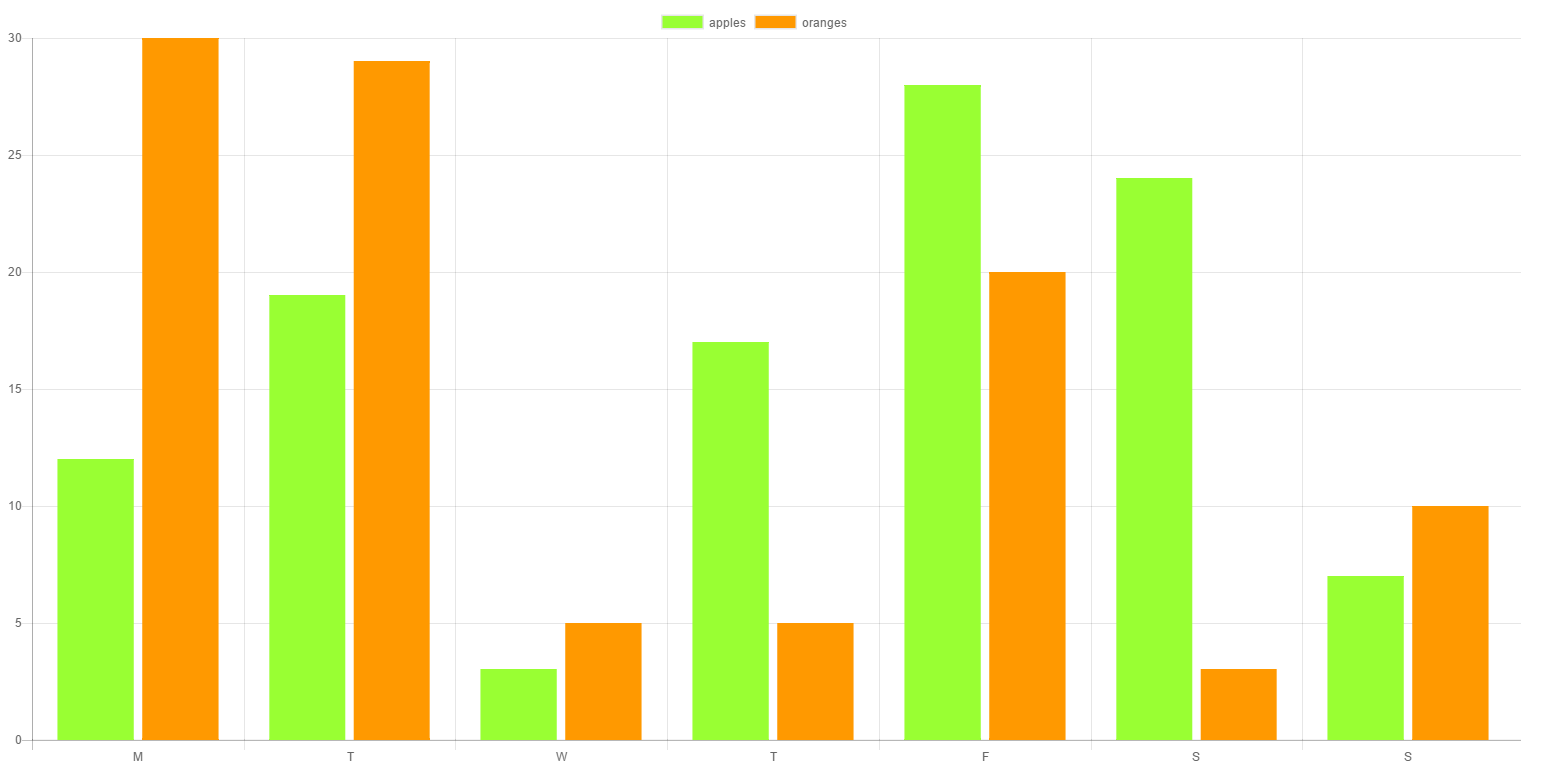
\includegraphics[width=5cm]{chart_bar} }}%
\subfloat[Spojnicový]{{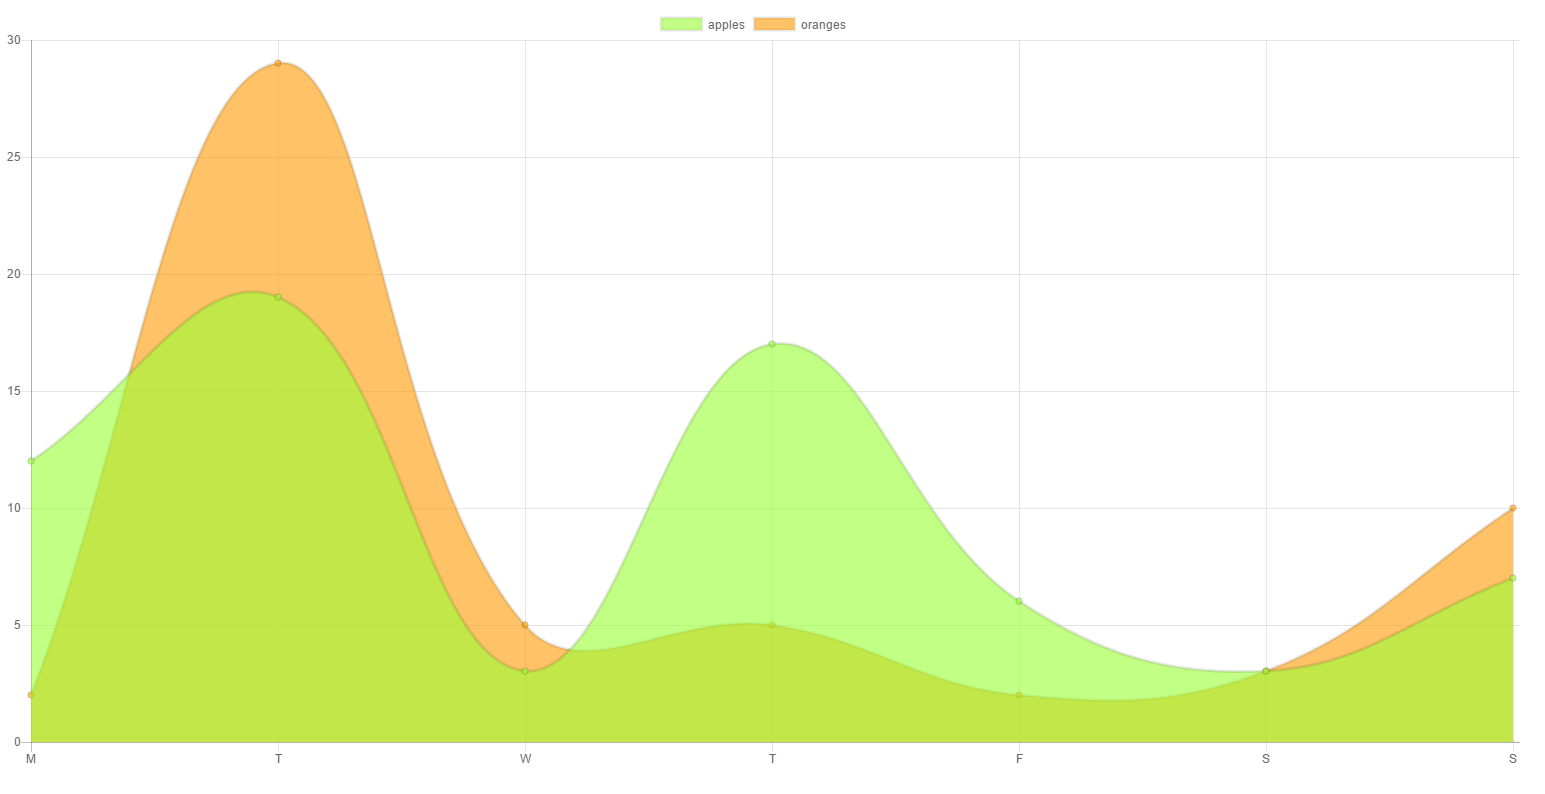
\includegraphics[width=5cm]{chart_line} }}%
\subfloat[Koláčový]{{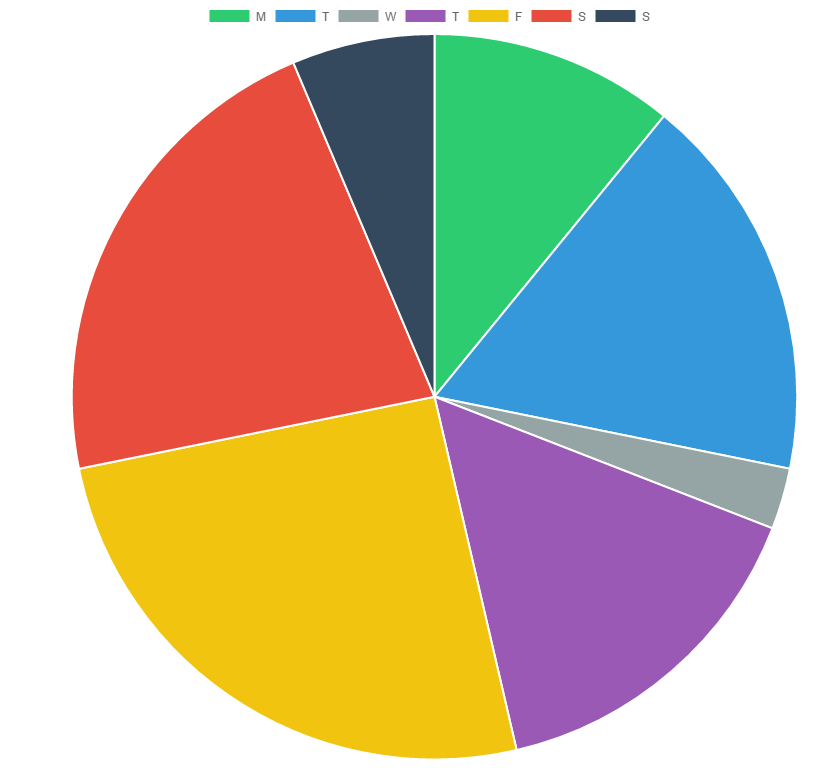
\includegraphics[width=5cm]{chart_pie} }}%
\caption{2 Figures side by side}%
\label{fig:example}%
\end{figure}

\subsubsection{Složitější grafy}
\par Jak již bylo nastíněno v předešlé sekci pro platící uživatele nabízí aplikace rozšířenou práci s grafy, převážně rozšíření typů grafů se kterými může uživatel pracovat. Také možnost exportovat grafy do formátu, který přečte aplikace Microsoft excel. Ale hlavní výhodou oproti jednoduchým grafům má použití knihovny D3, ta nabízí velké možnosti vytvoření jak grafů, tak různých grafických prvků. Tato knihovna je používaná nadstavbou \textbf{C3}, která definuje základní grafy, které je jednoduché vytvořit, ale je značně rozšiřitelná. Také v rámci složitější práce s grafy nabízíme uživateli možnost importovat data z různých formátů (CSV, XLS, XLSX atd.) a poté zvolit dokument do kterého se tato data vloží, případně pouze pracovat s těmito daty a vytvořit graf, který poté může uživatel uložit jako samostatnou entitu.

\subsection{Vyhledávací jazyk}
\par Vzhledem k tomu, že součástí požadavků na aplikaci bylo také možnost jednoduše filtrovat a hledat v jednotlivých entitách, museli jsme přijít s vyhledávacím jazykem, který pokryje jak složité vyhledávací dotazy, tak je pro uživatele jednoduchý pro pochopení.

\subsubsection{Z pohledu uživatelského rozhraní}
\par Pomocí uživatelského rozhraní může uživatel zadat vyhledávací text dvojím způsobem -- \textbf{Fulltext}, nebo \textbf{tokeny}.

\par Pokud zvolí fulltextové vyhledávání budou postupně uživateli napovídány jednotlivé texty napříč všemi entitami, tyto texty vytvoří nějaký způsobem větu, kterou odešleme na server a ten nám vrátí nejlépe sedící výsledky. Součástí této funkcionality je také postupné překreslování vyfiltrovaných entit, které se objevují pod vyhledávacím polem. V případě že se uživatel rozhodne vyhledávat pomocí tokenů usnadní serveru práci s odhadem co chce vyhledat a díky tomu dostane lépe sedící výsledky. Tokenizace probíhá tak, že si uživatel vybírá z předem definovaných prvků a na z těch je postupně tvořen dotaz na server. Opět, jak uživatel vytváří dotaz jsou mu předávány prvky které s velkou pravděpodobností hledá. Při použití tokenů uživatel získá také možnost hledat napříč několika entitami za použití logických operátorů, matematických (větší, rovno, menší než) a textových (podobnost) operandů.

\par Pokud se tedy podíváme na tyto dvě metody uživatel má možnost jednoduchého a rychlého hledání napříč aplikací pomocí fulltextového vyhledávání, nicméně toto vyhledávání není příliš vhodné pro složité dotazy. K tomuto slouží tokenové vyhledávání, které na druhou stranu je složitější, ale přináší možnost hledat napříč velkým množstvím entit. Jako bonus, uživatel si může tokenizované vyhledávání uložit jako filtr se jménem a následně v tokenizovaném filtru použít toto zástupné jméno. Může tedy postupně upravovat vnořené filtry, které může dále rozšiřovat a upravovat.

\subsubsection{Z pohledu serveru}
\par Pokud se zaměříme na vyhledávání z pohledu serveru musíme opět rozdělit tyto vyhledávací funkce na dvě části, stejně jako je tomu v případě uživatelského rozhraní.

\par Fulltextové vyhledávání je složitější pro server, převážně kvůli tomu, že jako dotaz bude mít vždy jeden dlouhý řetězec, který musí rozpadnout do jednotlivých prvků a nad těmi provést výsledné vyhledávání v rámci databáze. Server funguje tak, že si větu nejdříve rozdělí do jednotlivých slov a ty roztřídí do binárního stromu. Jak lze například vidět na obrázku \ref{binarni-strom}, kde je věta \textit{Restaurant in Brno with burger and pizza}. Server zpracovává binární strom od spodu a vždy když se mu povede vyhledat některý prvek označí větev za vyřešenou a již ji dále nezpracovává. Takže při použití tohoto příkladu server zjistí že uživatel hledá kolekci s názvem Restaurant, která obsahuje atribut Brno, dále server vyfiltruje všechny restaurace, které mají buger a které mají pizzu. Bohužel není vyhledávací algoritmus natolik přesný, aby vyhledal dokumenty ve kterých jsou tyto proměnné spojené.

\begin{figure}[!htb]
\centering
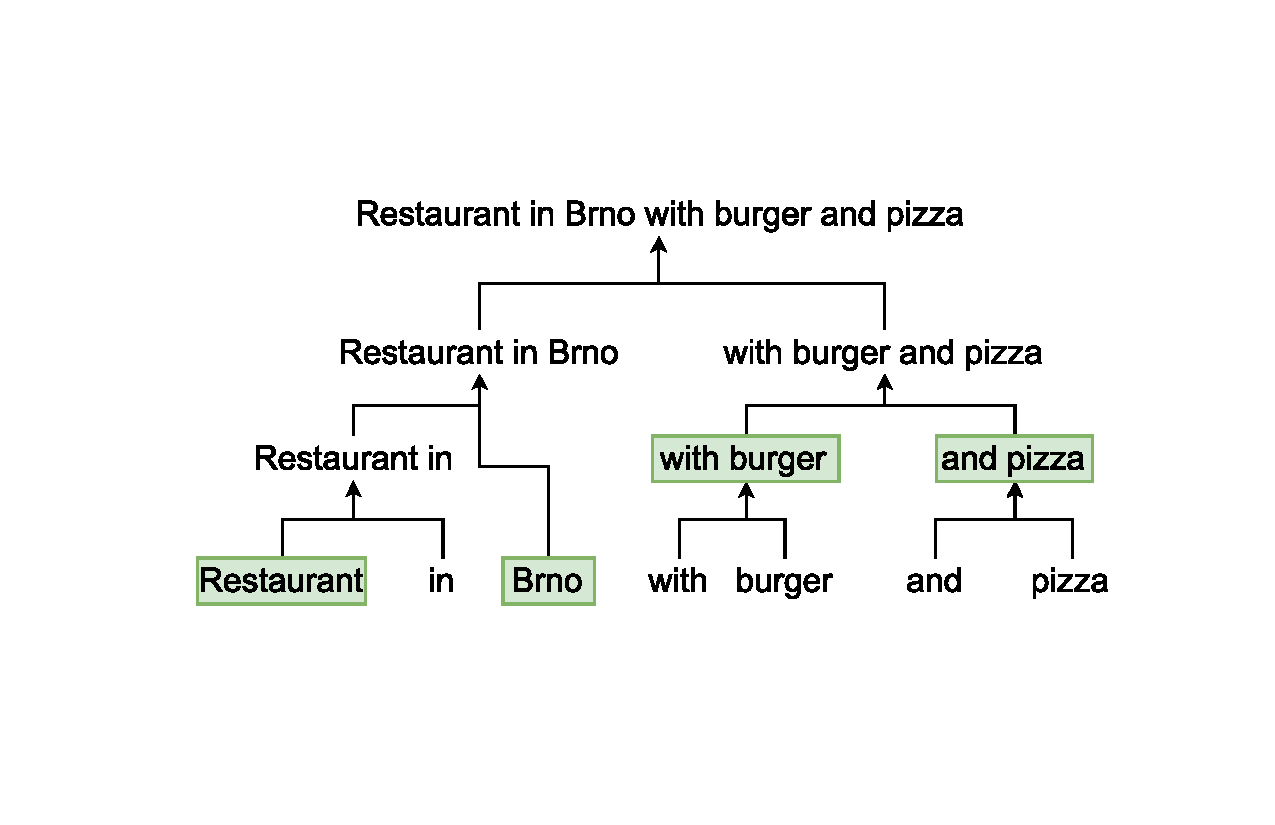
\includegraphics[max size={\textwidth}]{tree.pdf}
\caption{Binární strom pro roztřídění věty.}
\label{binarni-strom}
\end{figure}

\par Pokud uživatel použije tokenového vyhledávání usnadní tak serveru následné hledání, protože nemusí složitě rozdělovat větu a skládat ji do strojově srozumitelného vyhledávání. Pokud například vezmeme opět větu \textit{Restaurant in Brno with burger and pizza}, ta by v tekonové verzi vypadala tak, že by vyhledávací dotaz obsahoval čtyři tokeny každý s informací o jednotlivých požadavcích. Tokenizovaé vyhledávání si uživatel může uložit do takzvaných pohledů, které může následně vyhledávat (prokliknutím do něj se dostane rovnou na vyhledané entity skrz uložený dotaz) a používat ve vyhledávání.

\subsection{Zabezpečení}
\par V mnoha moderních aplikacích dochází k problémům se zabezpečením, ať již je to nedostatečné zabezpečení vůči případným útokům, tak nechtěného dovolení přístupu různým uživatelům k datům, ke kterým by neměli mít přístup. Tento nástroj se na toto téma snaží co nejvíce zacílit a použít řešení, které nebude příliš komplexní k nastavení pro zákazníka a zároveň bude poskytovat silné zabezpečení. Proto byl zvolen nástroj od firmy RedHat \textbf{Keycloak}, jehož fungování je popsáno v sekci o autentizačních serverech \ref{auth-server}.

\par V rámci tohoto nástroje je tento autentizační server nastaven tak, že před zapnutím aplikace je ověřeno přihlášení uživatele (díky nástroji Keycloak nemusí být uživatel přihlášen pouze k této aplikaci, ale k jakékoliv aplikaci spravované autentizačním serverem Keycloak, který má na starosti také tuto aplikaci). Pokud uživatel není přihlášen je vyzván k přihlášení, nabízíme možnost použít několik sociálních platforem -- Github, Facebook, Google účet a Twitter, kromě klasického přihlášení pomocí emailu a hesla. Poté se již každý dotaz na server kontroluje tímto autentizačním serverem, takže je možné nastavit jednoduše pravidla uživatelům pro přístup jak k RESTovým službám, tak jednotlivým zdrojům za pomoci Keycloak serveru a vytvořením skupin.

\par Díky autentizačnímu serveru se tedy v aplikaci nemusíme přímo starat o jednotlivé uživatele a nemusíme řešit zasílání hesel, celkovou správu a extra nastavení na serveru.

\section{Dolování dat}
\par Pokud vezmeme v úvahu hlavní modul starající se o dolování dat, můžeme ho rozdělit na tři části:
\begin{enumerate}
  \item \textbf{Heuristiky pro automatické linkování} -- pokud vznikne, nebo je upraven nějaký dokument je spuštěna řada automatických metod, které provedou případné automatické spojení.
  \item \textbf{Nejčastěji používané entity} -- na mnoha místech se aplikace snaží usnadnit práci uživateli tím, že mu nabídne ty, které jsou nejčastěji používané.
  \item \textbf{Přibližné napovídání} -- technika, která umožní napovídat uživateli možné výsledky při hledání bez nutnosti vyplnění celého jména.
\end{enumerate}

\subsection{Heuristiky pro automatické linkován}
\par Systém disponuje několika heuristikami, které se snaží vyhledávat skrytý význam v jednotlivých dokumentech a napomáhat tak uživateli při propojování dokumentů. Vezměme si například dva dokumenty -- jeden obsahuje jména, příjmení a telefonní čísla, nazvěme ho \textbf{uživatelský dokument}. Druhý bude například \textbf{studentský dokument}, ten bude obsahovat spojená jména a příjmení studentů spolu s jejich celkovým prospěchem. Po vytvoření studentského dokumentu nemusí mít uživatel tušení, že existuje uživatelský dokument a nevytvoří tak manuální propojení, nicméně systém si označí tyto dva dokumenty jako potencionální spojení a při zadávání dat do dokumentu studentů nám bude napovídat jména a příjmení z uživatelského dokumentu. Propojení těchto dokumentů tedy vznikne automaticky. Uživatel o tomto propojení nemusí být nijak informován, ale na stránce detailu studentského dokumentu uvidí informativní hlášku, která mu sdělí, že vzniklo nové propojení. Tento link může dále uživatel upravit, případně ho může odstranit a systém mu již nebude napovídat jména a příjmení.

\par Toto automatické propojení vzniká na základě dvou heuristických technik a následného vyhodnocení pomocí složení dvou sloupců z jedné tabulky do druhé. Tímto docílíme jednoduchosti a hlavně rychlosti zadávání nových záznamů. Velkou výhodou této techniky je, že sloupce, které jsou označeny jako propojené a získávané z různých tabulek, se automaticky obnovují, takže v případě změny jména v souboru uživatelů se tato změna automaticky projeví také ve studentském dokumentu (opět lze tuto funkci vypnout pro celý dokument, případně pro jednotlivé záznamy).

\par Nad takto nově vzniklými propojeními lze provádět samozřejmě stejné operace jako v případě klasických propojení -- tedy definovat propojovací řetězec a jednoduché funkce. Nicméně při vytvoření jednoduchých funkcí uživatel bohužel ztrácí automatické znovunačtení záznamů. Pokud chce načíst změny v takových záznamech, musí si vyžádat načtení hodnot, které jsou následně uloženy do souboru.

\par Příklady takových propojení můžeme vidět na obrázku \ref{linkovani}, kde první tabulka s názvem Nabízené zboží získává data ze dvou tabulek a poté další tabulka o (Věk a pohlaví uživatelů) čerpá jména z dokumentu, který obsahuje všechna možná jména.

\begin{figure}[htp]
\centering
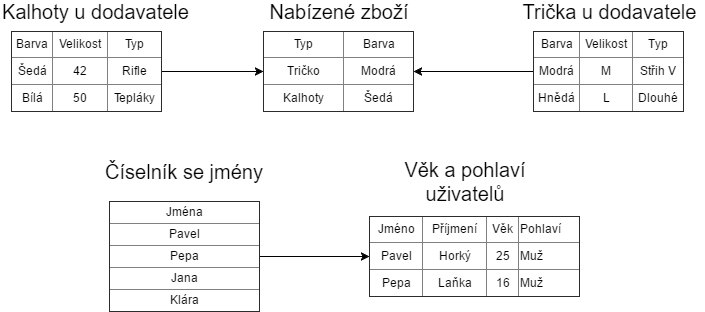
\includegraphics[max size={\textwidth}]{linkovani}
\caption{Příklad automaticky prolinkovaných dokumentů.}
\label{linkovani}
\end{figure}

\subsubsection{Heuristika 1}
\par V případě první heuristiky se kontrolují pouze záhlaví tabulky, takže pokud vezmeme v úvahu definovaný příklad, v momentě vytvoření dokumentu se provede kontrola nad podobnými soubory, a pokud se najde shoda, propojení se automaticky vytvoří.
\subsubsection{Heuristika 2}
\par Tato heuristika je složitější a znamená velkou zátěž pro systém, proto je potřeba dopředu provést nastavení tabulky při vytváření. Funguje tak, že při vytvoření nové tabulky uživatel může definovat tuto tabulku jako zdrojové data a kdykoliv se bude vytvářet nový soubor, provede se kontrola nad zdrojovými tabulkami, zda některá neobsahuje příslušný záznam. Vzhledem k náročnosti na systém jsme se rozhodli, že tuto vlastnost odstupňujeme pro jednotlivé druhy zákazníků.

\subsection{Nejčastěji používané entity}
\par S přihlédnutím k uživatelským požadavkům obsahuje systém možnost zobrazit entity, které jsou nejčastěji používané daným uživatelem pro jednu organizaci a projekt. Pro zobrazení požadovaných entit jsme nejdříve vybrali algoritmus \textbf{fronta}, ale tento model se nám neosvědčil, protože se často stávalo, že nejpoužívanější entity mizely z rychlého výberu a méně časté se nacházely v nabídce, proto jsme do systému naimplementovali možnost přepnutí na takzvanou \textbf{frontu s počítadlem} -- možnost pouze pro zákazníky s kvalitnější podporou. Přepnutí těchto technik se poté nachází v uživatelském nastavení, takže každý uživatel je schopen si toto řazení změnit.

\subsubsection{Fronta}
\par Fronta funguje na stylu omezeného počtu záznamů, které mohou být zobrazeny, a pokud je tento počet překročen, poslední záznam, který byl zaktivován, je odstraněn. Toto řešení je dostačující, nicméně může nastat to, že entita, která je často otevíraná, zmizí z tohoto seznamu kvůli otevření několika stejných entit. Chování v aplikaci lze vidět na obrázku \ref{zasobnik}, kdy fronta obsahuje entity označené 1, 2, 3, 4 a 5. Uživatel otevřel nově entitu s označením c a entity v zásobníku jsou tedy (od spodu fronty) c, 1, 2, 3 a 4.
\begin{figure}[htp]
\centering
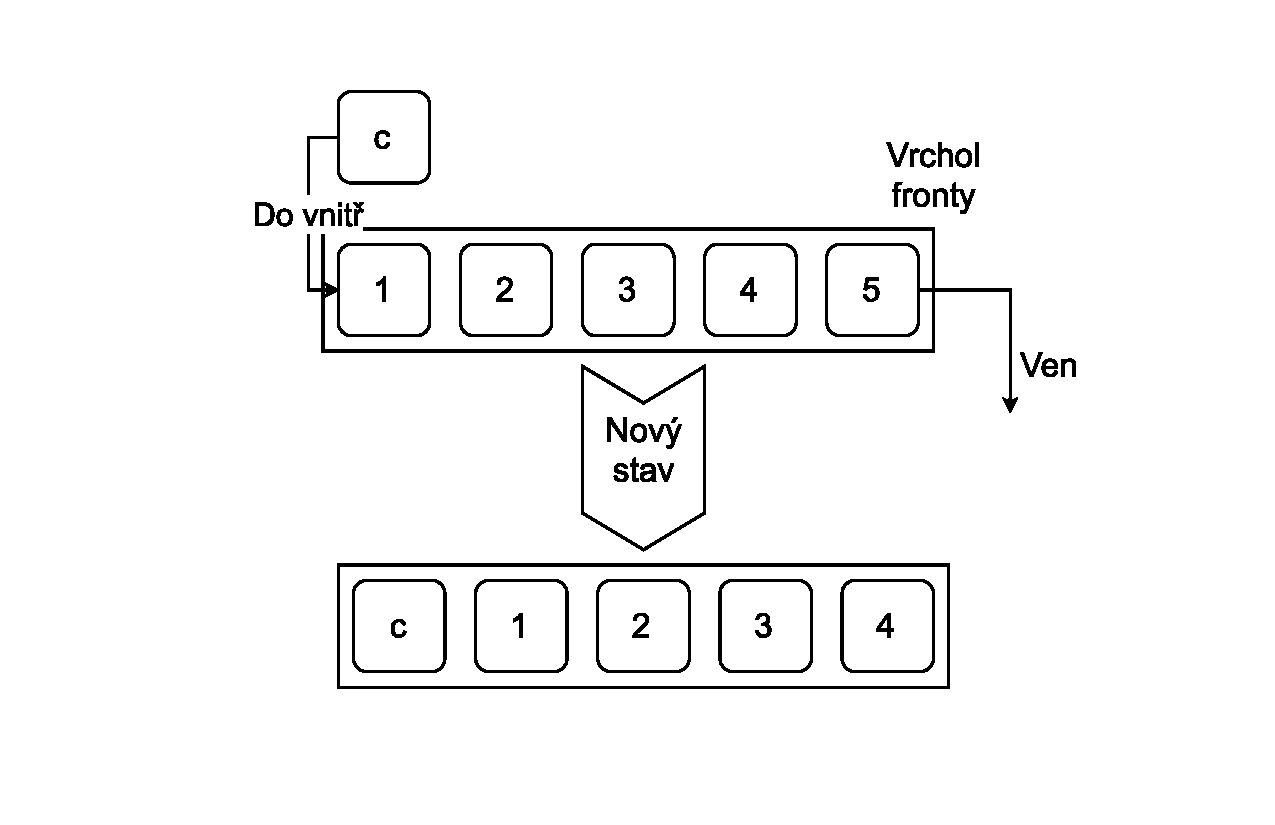
\includegraphics[max size={\textwidth}]{zasobnik.pdf}
\caption{Příklad plnění jednoduché fronty.}
\label{zasobnik}
\end{figure}

\subsubsection{Fronta s počítadlem}
\par Fronta s počítadlem je v podstatě rozšířená implementace fronty. Pokud je některá entita otevíraná častěji, je u ní zvyšován počet otevření. Entita s největším počtem otevření je na spodu fronty a entita s nejmenším počtem navrchu. Pokud se otevře nový dokument, je mu zvýšen počet otevření, a pokud překročí toto číslo nejvrchnější prvek ve frontě, tato nově otevřená entita nahradí tu, která byla na vrcholu fronty. Provedeno v rámci aplikace můžeme vidět na obrázku \ref{counter} -- nejčastěji používaná entita je označena 2 a nejméně používaná je označena 5; dále uživatel otevřel nově dokument s označením c a poté otevřel dokument d, který byl předtím otevřen jednou. Nově tedy zásobník obsahuje entity 2, 3, 4, 1 a d.
\begin{figure}[htp]
\centering
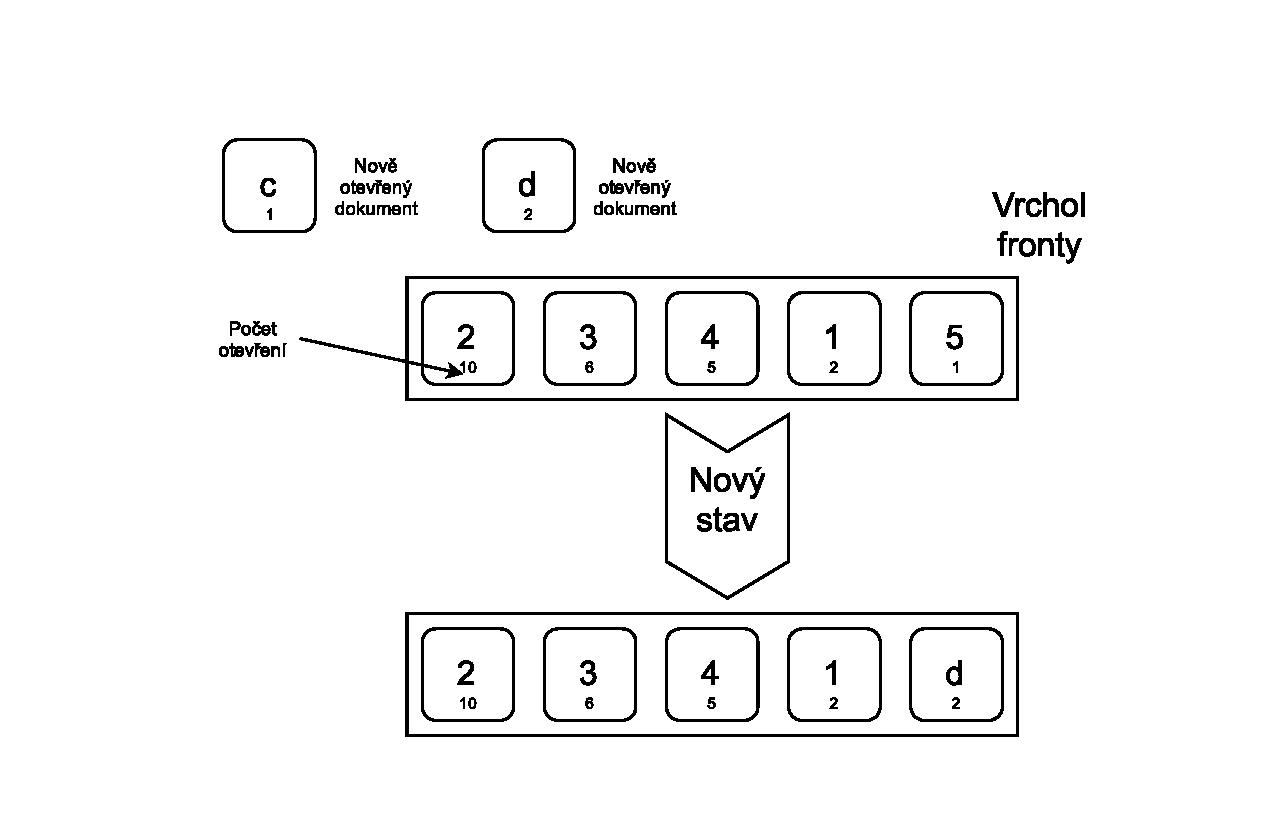
\includegraphics[max size={\textwidth}]{rozsireny-zasobnik.pdf}
\caption{Příklad plnění rozšířené fronty s počítadlem.}
\label{counter}
\end{figure}

\subsection{Přibližné napovídání}
\par Přibližné napovídání pracuje nad takzvanou fuzzy logikou a funguje na principu, že zadaný řetězec nemusí být vždy přesně zadán, aby uživateli byl dodán výsledek, který požaduje. Přibližné napovídání v aplikaci přibližné napovídání funguje tak, že v momentě, kdy uživatel zadá hledaný řetězec, jsou mu zobrazeny záznamy, které se nejblíže shodují k danému řetězci (případně obsahují prvních pár písmen), ideálně jsou tyto řetězce shodné. Aplikace nabízí možnost zobrazit uživateli entity, které mají v názvu nebo v možných řetězcích jedno písmeno jiné. Pokud uživatel následně vybere entitu, je k ní tento hledaný řetězec přidán. Entita tedy obsahuje seznam možných hledaných řetězců, které se dále mohou lišit o jedno písmeno. Například pokud budeme hledat entitu s názvem \textbf{Restaurace}, tato entita dále obsahuje seznam možných hledaných řetězců -- například \textit{Rez}, \textit{taue}, \textit{auea} a \textit{Res}. Uživatel tak zadá do hledání \textbf{Restaues} a systém mu nabídne entitu \textbf{Restaurace}.

\section{Analýza rizik}
\par Vzhledem k tomu, že vytvořit náročnou aplikaci není triviální, na začátku vývoje jsme si vytvořili analýzu možných rizik, na která můžeme narazit během vývoje a při distribuci. Také jsme si tato rizika ohodnotili a pro některé, které by měli vysoký dopad na aplikaci, jsme si připravili riziková opatření.

\par Následující tabulky znázorňují pravděpodobnost výskytu a dopad rizika.
\begin{table}[!htb]
    \begin{minipage}{.5\linewidth}
      \centering
\begin{tabular}{|c | c |}
\hline
Pravděpodobnost&Hodnota\\
\hline
0 - 20 \%&1\\
\hline
20 - 40 \%&2\\
\hline
40 - 60 \%&3\\
\hline
60 - 80 \%&4\\
\hline
80 - 100 \%&5\\
\hline
\end{tabular}
    \end{minipage}%
    \begin{minipage}{.5\linewidth}
      \centering

\begin{tabular}{|c | c |}
\hline
Hodnota&Dopad\\
\hline
1&Velmi nízký\\
\hline
2&Nízký\\
\hline
3&Střední\\
\hline
4&Vysoký\\
\hline
5&Velmi vysoký\\
\hline
\end{tabular}
    \end{minipage} 
    \caption{Ohodnocení pravděpodobnosti a dopadu rizika.}
\end{table}

\par Po vytvoření základních tabulek pro odhadnutí rizik jsme jednotlivá rizika zapsali do tabulky a ohodnotili jsme je možnou pravděpodobností a dopadem na funkčnost, nasazení nebo nepřijetí uživateli. jako mezní hodnotu jsme si určili 14 bodů při ohodnocení pravděpodobnosti a dopadu rizika -- výsledek je možné vidět v tabulce \ref{rizika}.

\begin{longtable}{ || c || m{3cm} | m{4cm} | c | c | c | c | }
\hline
Č. & Scénář & Hrozba & Pravděp. & Dopad & Hodnocení\footnote{Hodnocení = Pravděpodobnost * Dopad.}\\
\hline
\endhead
1 & Pomalý vývoj & S příchodem zákazníků budou přibývat požadavky na systém, které nemusíme stíhat přidávat & 2 & 3 & 6 \\
\hline
2 & Uživatelé nebudou rozumět aplikaci & Uživatelské rozhraní nebude intuitivní a snadno ovladatelné & 3 & 3 & 9 \\
\hline
3 & Nezabezpečená data & Kdokoli se dostane k uživatelským datům & 3 & 5 & \cellcolor{red!55}15 \\
\hline
4 & Napadení aplikace & Napadení aplikace třetí stranou & 2 & 5 & 10 \\
\hline
5 & Pomalá práce s daty & Při velkém objemu dat může nastat zamrzání aplikace & 4 & 3 & \cellcolor{yellow!55}12 \\
\hline
6 & Nezájem investorů & Aplikace nezujme případné investory, což povede k nedostatku zdrojů v prvotním spuštění & 3 & 5 & \cellcolor{red!55}15 \\
\hline
\caption{Možné scénáře rizik při vývoji a nasazení.}
\label{rizika}
\end{longtable}

\par Jak lze vidět v tabulce \ref{rizika}, tak pouze 2 rizika si vyžadují speciální pozornost, protože překračují námi definovanou hranici. Zaměříme se také na riziko s číslem \textbf{5}, které by mělo také kritický dopad na chod aplikace.

\begin{longtable}{ || c || m{3cm} | m{4cm} | c | c | c | c | }
\hline
Č. & Opatření & Cena & Pravděp.\_ & Dopad\_ & Hodnocení\_\footnote{Hodnocení = Pravděpodobnost\_ * Dopad.\_} \\
\hline
\endhead
3 & Při vývoji použijeme nástroj, který zabezpečí data & Cena nástroje pro zabezpečení & 2 & 5 & 10 \\
\hline
5 & Použití indexovacího nástroje & Cena nástroje pro indexaci dat & 3 & 3 & 9 \\
\hline
6 & Dedikování člověka pro komunikaci s investory & Cena člověka pro komunikaci & 2 & 5 & 10 \\
\hline
\caption{Opatření pro vyhnutí rizikům.}
\label{rizika}
\end{longtable}

\par Z možných opatření vyplývá že všem potencionálním technickým rizikům, ktera by měla vysoký dopad, se dá vyhnout použitím vhodných technologií a v případě rizika \textbf{6}, které by znamenalo možný nezájem investorů, musíme dedikovat člověka pro komunikaci a vytváření povědomí o tomto nástroji.

\par Pro znázornění zavedení opatření pro vyhnutí rizik jsme zvolili terčový graf \ref{risk-graph}, na kterém lze vidět, že žádné riziko nepřekračuje hodnotu 14 bodů, kteréou jsme si nastavili jako kritický bod. Nevěnovali jsme se rizikům, která nemají tak vysokou pravděpodobnost, že by nastala, nicméně i na ta je třeba dávat si pozor, a proto je dobré, že jsme na některá z nich narazili již na začátku.

\begin{graph}[ht]
\centering
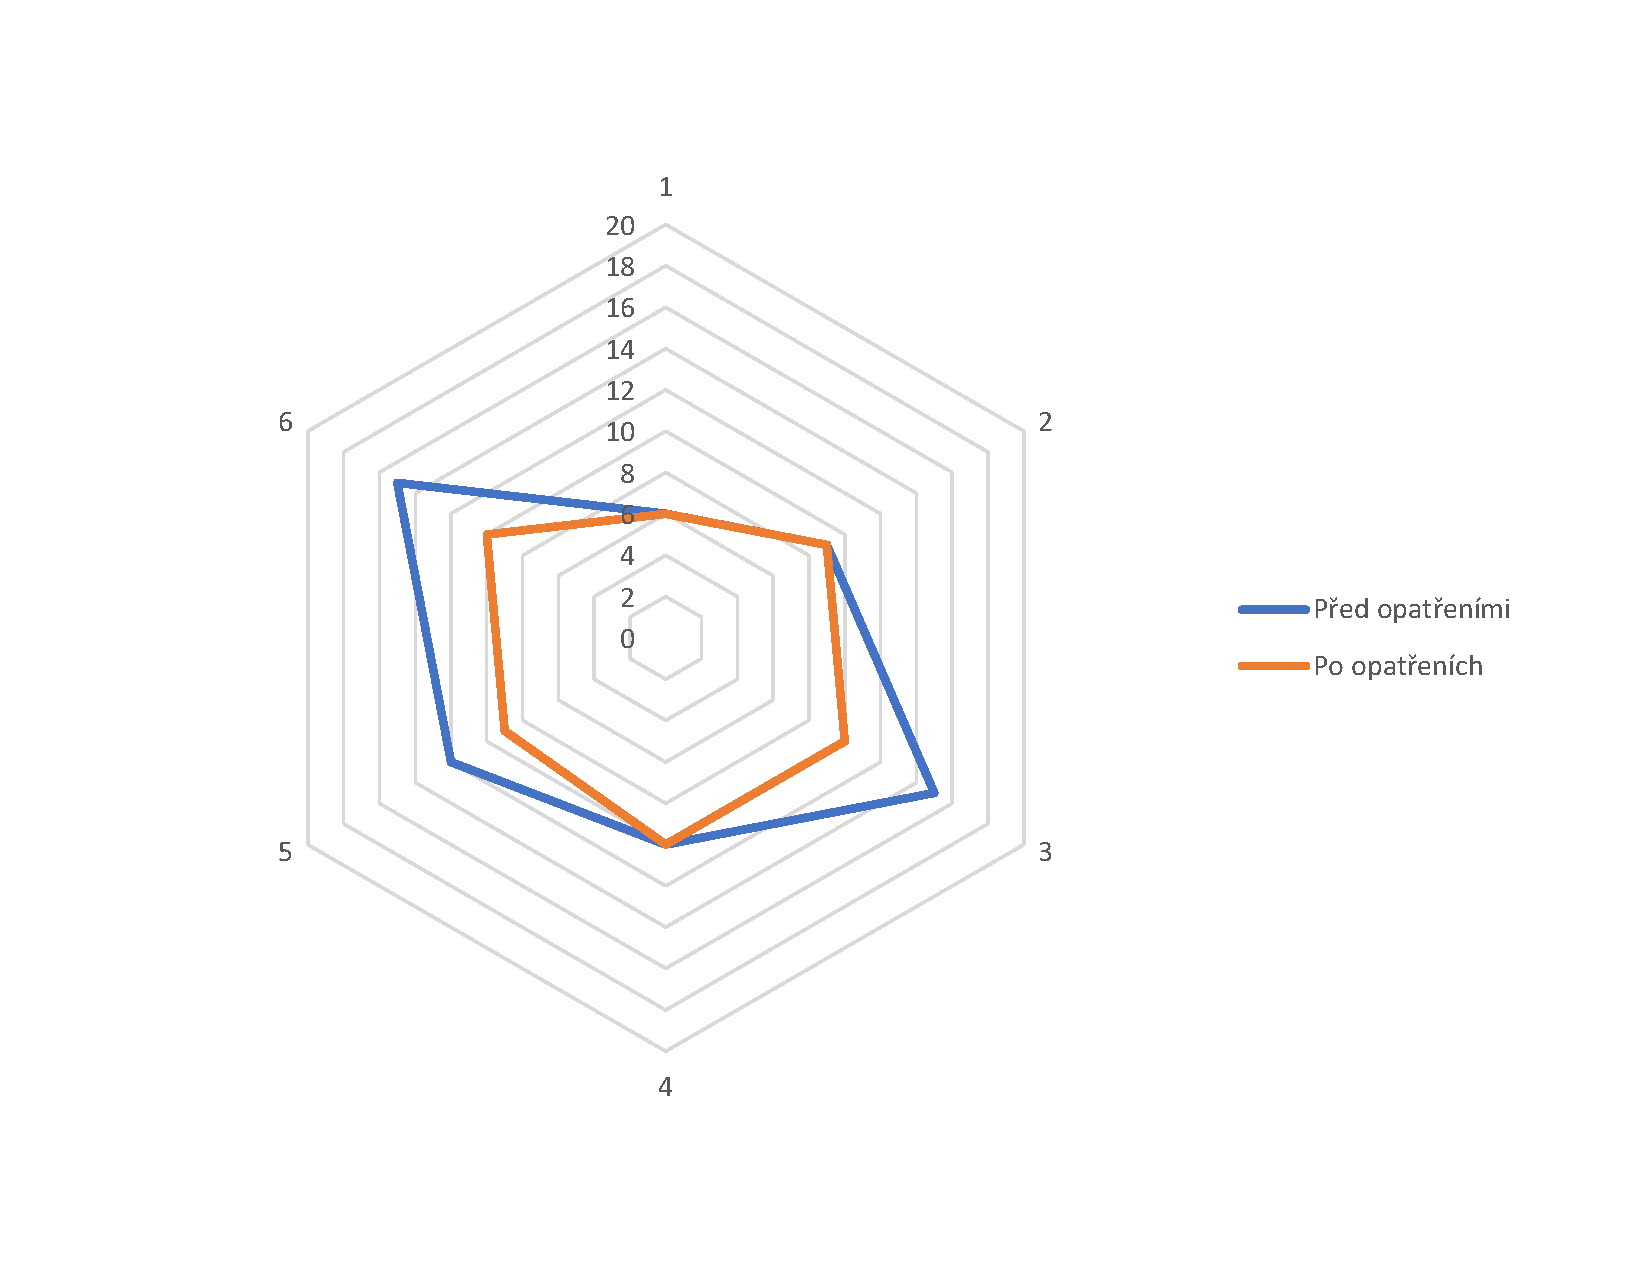
\includegraphics[max size={\textwidth}]{graph.pdf}
\caption{Rizika před a po zavedení rizikových opatření.}
\label{risk-graph}
\end{graph}

\section{Cenový model}
\par Jak již bylo několikrát řečeno v předchozím textu, aplikace se bude nabízet v několika cenových relacích, kdy více platící zákazníci dostanou na výběr větší množství funkcí a také větší podporu od vývojového týmu.

\par Cenový model můžeme shrnout do tří skupin -- \textbf{základní}, \textbf{střední} a \textbf{nejvyšší} (označováno též jako stříbrný, zlatý a platinový zákazník). Zákazníci si sami vyberou, jaké funkcionality se jim více hodí, přičemž první 2 měsíce mají zdarma na vyzkoušení. Takže zákazník dostane na začátku plnou podporu všech funkcí systému bez nutnosti platit jakoukoliv částku. V případě, že by chtěl školení, případně lepší podporu v těchto dvou měsících, je s ním vytvořena speciální smlouva, která může pokrývat tyto dva zkušební měsíce. Pokud nechce na začátku zákazník nic platit, nemusí, dostane návod jak aplikaci používat a menší ukázku toho, co s aplikací dělat a má možnost dva měsíce bezplatně testovat tento produkt.

\par Po uplynutí dvouměsíční lhůty si zákazník sjedná schůzku, kde se domluví bližší detaily přechodu do systému. Na začátku zákazník platí za služby jako například převod celé databáze, školení uživatelů, podporu při problémech a výpadcích atd. Každý úkon je ohodnocen individuálně na základě velikosti databáze (případně počtu uživatelů a jejich požadavků) a době strávené na přechodu pod systém.

\par Pokud zákazník souhlasí se všemi podmínkami a je ochotný začít používat aplikaci, je s ním také vytvořen speciální platící plán, ve kterém záleží na počtu uživatelů, kteří budou mít přístup k systému a k funkcionalitám, které jednotliví uživatelé požadují. Tento platící plán je opět individuální a nejvíce se mění v závislosti na počtu a druhu aktivovaných funkcí a na skupině zákazníka.

\par Vzhledem k tomu, že vývoj aplikace probíhá formou open-source, nemáme možnost, aby si schopnější uživatelé nevzali vyvýjenou aplikaci a nespustili si ji sami na svém vlastním stroji, tomuto se nijak nebráníme a je jasné, že takové případy budou vznikat, proto musíme sázet na to, že zákazníci budou chtít platit za podporu a za přidané hodnoty, na které mají nárok v rámci cenových modelů.
